\documentclass[12pt]{article}
\usepackage{notes-common}
\usepackage{graphicx}
\geometry{margin=0.35in}
\AtBeginDocument{\fontsize{14}{17}\selectfont}

% Complete / filled-in reference version of cyclotron-helix-notes.tex.
% Fri Oct 30 -- Magnetic force on moving charges (Knight 29.7). Sec.2 is
% Knight Example 29.11 (electron accelerated through 500 V, then injected
% into a uniform field; find the field's strength from the half-revolution
% time, then the orbit radius). Sec.3 is a new (not-from-the-book) problem:
% split v into components parallel/perpendicular to B to get helical
% motion, then find both the helix radius and the pitch.
\newcommand{\eqline}[2][-0.5mm]{%
  \par\vspace{1mm}\noindent #2\par\vspace{#1}%
  \noindent\textcolor{rulehue}{\rule{\linewidth}{0.5pt}}\par\vspace{4mm}%
}
\newcommand{\ANS}[1]{\textcolor{accent}{#1}}

\begin{document}

\noteshead{Magnetic Force on Moving Charges \textcolor{accent}{(completed)}}{}

\goal{
\begin{itemize}[itemsep=5pt,parsep=2pt,topsep=2pt]
\item See why a charge moving across a uniform $\vec B$ field goes in a
circle, and where the cyclotron radius $r=mv/|q|B$ comes from.
\item Work a full numerical example end to end: accelerate a charge through
a potential difference, then find the field strength from how fast it
circles (Example 29.11).
\item Split $\vec v$ into the piece along $\vec B$ (untouched) and the piece
across it (circles), to see why a charge entering at an angle traces a
\emph{helix}, not a circle.
\item Find both the radius of that helix and its \emph{pitch} --- the
distance the charge drifts along $\vec B$ during one full loop.
\end{itemize}}

%============================================================
\nsec{Why a uniform field makes a charge go in a circle}

A charge $q$ moves with speed $v$ perpendicular to a uniform field $\vec B$.
The magnetic force $\vec F=q\vec v\times\vec B$ is always perpendicular to
$\vec v$ --- it only ever turns the velocity, never speeds it up or slows it
down. A force that's always perpendicular to the motion, with constant
magnitude, is exactly what produces \ANS{uniform circular} motion.

Set the magnetic force equal to the centripetal force it's providing:

\[
|q|\,v\,B \ =\ \ANS{\dfrac{mv^2}{r}}
\]
\vspace{0.8cm}

Solve for the radius of the circle:

\result[1.6cm]{$r_{\text{cyc}} = \ANS{\dfrac{mv}{|q|B}}$}

\checkpoint{Does a \emph{faster} charge circle in a bigger or smaller
radius? Does a \emph{stronger} field give a bigger or smaller radius? Is
either answer the opposite of what you expected?}

{\small\color{accent} Faster $\Rightarrow$ bigger radius ($r\propto v$).
Stronger field $\Rightarrow$ smaller radius ($r\propto 1/B$) --- a stronger
field turns the charge \emph{more sharply}, not less. That second one trips
people up if they picture a stronger field as a ``bigger push'' that would
fling the charge outward; instead it's a tighter leash.}

%============================================================
\nsec{Worked example: the radius of cyclotron motion}

\textit{Example 29.11. An electron is accelerated from rest through a
potential difference of $500$ V, then injected into a uniform magnetic
field. Once in the field, it completes half a revolution in $2.0$ ns. What
is the radius of its orbit?}

\begin{center}
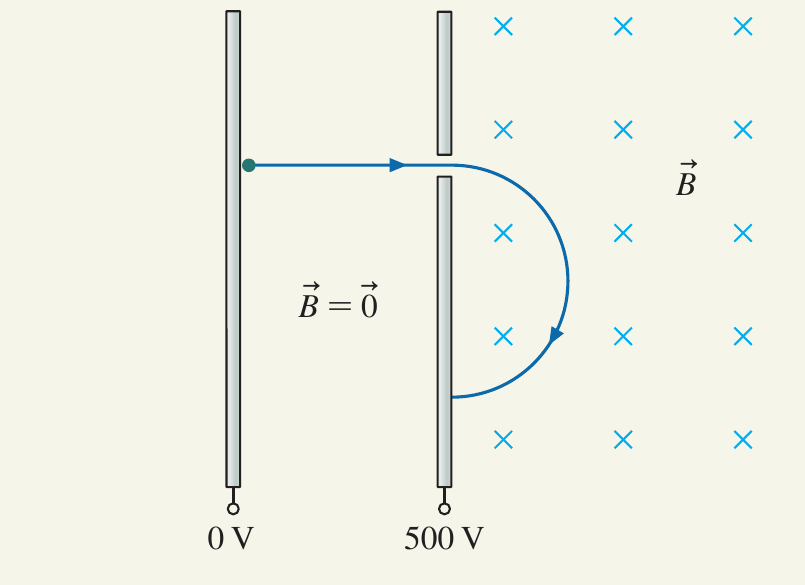
\includegraphics[width=0.52\linewidth]{figures/knight-fig29-38.png}
\end{center}
\figtask{Label the $0$ V and $500$ V plates, mark $\vec B$'s direction, and
sketch the electron's path: straight across the gap, then curving once it
enters the field.}

\textbf{Step 1 --- speed entering the field.} Energy conservation,
$K_f+qV_f=K_i+qV_i$, with $K_i=0$:

\[
\tfrac12 m v_f^2 = e\,V_f \qquad\Longrightarrow\qquad v_f = \ANS{\sqrt{\dfrac{2eV_f}{m}}}
\]
\vspace{1.0cm}

\eqline[0.2cm]{$v_f = \ANS{1.33\times10^{7}\text{ m/s}}$}

\textbf{Step 2 --- turn the half-revolution time into a period and
frequency.} Half a revolution takes $2.0$ ns, so a full revolution (the
period $T$) takes \ANS{$4.0$ ns}. The cyclotron frequency is
$f=1/T=\ANS{2.5\times10^8\text{ Hz}}$.

\textbf{Step 3 --- use the cyclotron frequency to get $B$.} The cyclotron
frequency doesn't depend on $v$ or $r$ at all:

\[
f = \dfrac{|q|B}{2\pi m} \qquad\Longrightarrow\qquad B = \ANS{\dfrac{2\pi m f}{e}}
\]
\vspace{1.0cm}

\eqline[0.2cm]{$B = \ANS{8.94\times10^{-3}\text{ T}}$}

\textbf{Step 4 --- now find the radius}, using $v_f$ from Step 1 and $B$
from Step 3:

\result[1.6cm]{$r_{\text{cyc}} = \dfrac{mv_f}{eB} = \ANS{8.5\times10^{-3}\text{ m} = 8.5\text{ mm}}$}

\checkpoint{The review in the book compares this radius to a photo of an
electron beam curving in a magnetic field. Does $8.5$ mm sound like a
reasonable size for an electron's orbit in a lab-scale field, or suspiciously
large/small?}

{\small\color{accent} Reasonable --- a 17-mm-\emph{diameter} orbit is the
kind of thing you can actually see curve in a tabletop electron-beam tube.
If this had come out at, say, $8.5$ \emph{nm} or $8.5$ km, that would be the
signal to go back and check a power of ten.}

%============================================================
\nsec{When $\vec v$ isn't perpendicular to $\vec B$: helical motion}

Every example so far has had $\vec v\perp\vec B$ exactly. What if the charge
enters at some other angle $\theta$ to the field?

Split $\vec v$ into two pieces, one along $\vec B$ and one across it:

\[
\vec v = \vec v_\parallel + \vec v_\perp\,, \qquad
v_\parallel = v\cos\theta\,, \qquad v_\perp = v\sin\theta
\]

\begin{center}
\begin{tikzpicture}[x=1cm,y=1cm]
  \draw[-latex, gray, line width=1pt] (-0.3,0) -- (2.4,0) node[right,scale=0.8]{$\vec B$};
  \draw[-latex, accent, line width=1.2pt] (0,0) -- (1.6,1.2) node[above,scale=0.8]{$\vec v$};
  \draw[dashed, gray] (1.6,1.2) -- (1.6,0);
  \draw[-latex, blue!55!black, line width=1pt] (0,0) -- (1.6,0) node[below,scale=0.75]{$v_\parallel$};
  \draw[-latex, red!60!black, line width=1pt] (1.6,0) -- (1.6,1.2) node[right,scale=0.75]{$v_\perp$};
  \draw (0.45,0) arc (0:36.5:0.45);
  \node[scale=0.7] at (0.68,0.16) {$\theta$};
\end{tikzpicture}
\end{center}

\begin{itemize}[itemsep=6pt,parsep=3pt,topsep=3pt]
\item The parallel piece, $\vec v_\parallel$, is \ANS{parallel (or
anti-parallel)} to $\vec B$ --- so $\vec v_\parallel\times\vec B=0$:
\ANS{zero} force at all. Left alone, it just \ANS{drifts at constant
velocity along $\vec B$, forever}.
\item The perpendicular piece, $v_\perp$, is exactly \S1's situation all
over again --- it circles with radius $\ANS{r=\dfrac{mv_\perp}{|q|B}}$ (the
\S1 formula, with $v_\perp$ in place of $v$).
\end{itemize}

Put the two motions together --- a uniform drift along $\vec B$, plus a
circle in the plane across $\vec B$ --- and the path traced out is a
\ANS{helix}: a \ANS{corkscrew / spring-shaped path that advances steadily
along $\vec B$ while circling around it}.

\checkpoint{At $\theta=90^\circ$ you're back to \S1's pure circle. What does
the path look like in the other extreme, $\theta=0^\circ$?}

{\small\color{accent} At $\theta=0^\circ$, $v_\perp=0$ --- there's no
circling at all, and the charge just travels in a straight line along
$\vec B$ at constant speed $v$. A straight line is the $\theta\to0$ limit of
a helix with the pitch stretched out to infinity (zero radius).}

\textit{New problem. A proton ($m=1.67\times10^{-27}$ kg, $q=+e=
1.60\times10^{-19}$ C) enters a region of uniform magnetic field
$B=0.50$ T. Its velocity has magnitude $v=4.0\times10^5$ m/s and points
$30^\circ$ away from $\vec B$. Find (a) the radius of the helix it traces,
and (b) the \emph{pitch} --- the distance it drifts along $\vec B$ during
one full revolution.}

\begin{center}
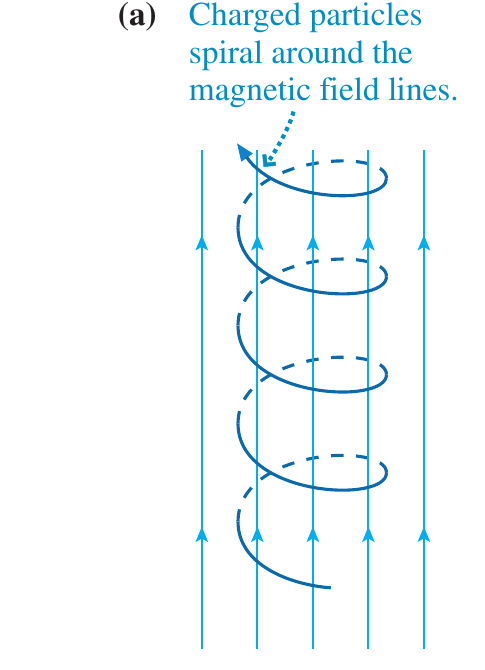
\includegraphics[height=5.4cm]{figures/knight-fig29-39a.png}
\end{center}
\figtask{Mark one full turn of the helix and label the pitch you're solving
for.}

\textbf{Step 1 --- components of $v$ relative to $\vec B$}:

$v_\parallel = v\cos30^\circ = $ \ANS{$3.46\times10^5$ m/s} \qquad
$v_\perp = v\sin30^\circ = $ \ANS{$2.0\times10^5$ m/s}

\textbf{Step 2 --- radius of the helix} (same formula as \S1, using
$v_\perp$):

\result[1.6cm]{$r_{\text{helix}} = \dfrac{mv_\perp}{qB} = \ANS{4.2\times10^{-3}\text{ m} = 4.2\text{ mm}}$}

\textbf{Step 3 --- period of one full revolution} (this doesn't depend on
$v_\perp$ at all --- why not? see \S1):

\[
T = \dfrac{2\pi m}{qB} = \ANS{1.31\times10^{-7}\text{ s} = 131\text{ ns}}
\]
\vspace{1.0cm}

\eqline[0.2cm]{$T = \ANS{1.31\times10^{-7}\text{ s}}$}

\textbf{Step 4 --- the pitch.} During one period $T$, the parallel motion
just moves at constant velocity $v_\parallel$:

\result[1.6cm]{$\text{pitch} = v_\parallel\,T = \ANS{4.5\times10^{-2}\text{ m} = 4.5\text{ cm}}$}

\checkpoint{If the proton had instead entered at a \emph{smaller} angle
$\theta$ (closer to parallel with $\vec B$), would the helix get fatter or
skinnier? Would it get more tightly or more loosely wound (bigger or
smaller pitch)?}

{\small\color{accent} Smaller $\theta$ means less of $v$ is perpendicular
($v_\perp=v\sin\theta$ shrinks), so the helix gets \emph{skinnier}
(smaller radius). At the same time more of $v$ is parallel
($v_\parallel=v\cos\theta$ grows), so the pitch grows too --- the helix gets
\emph{more loosely wound}. (The period $T$ itself doesn't change at all ---
it never depended on $\theta$.)}

\end{document}
